%%%%%%%%%%%%%%%%%%%%%%%%%%%%%%%%%%%%%%%%%
% Beamer Presentation
% LaTeX Template
% Version 1.0 (10/11/12)
%
% This template has been downloaded from:
% http://www.LaTeXTemplates.com
%
% License:
% CC BY-NC-SA 3.0 (http://creativecommons.org/licenses/by-nc-sa/3.0/)
%
%%%%%%%%%%%%%%%%%%%%%%%%%%%%%%%%%%%%%%%%%

%----------------------------------------------------------------------------------------
%	PACKAGES AND THEMES
%----------------------------------------------------------------------------------------

\documentclass{beamer}
\usepackage[french]{babel}
\usepackage[utf8]{inputenc}

\mode<presentation> {

% The Beamer class comes with a number of default slide themes
% which change the colors and layouts of slides. Below this is a list
% of all the themes, uncomment each in turn to see what they look like.

%\usetheme{default}
%\usetheme{AnnArbor}
%\usetheme{Antibes}
%\usetheme{Bergen}
%\usetheme{Berkeley}
%\usetheme{Berlin}
%\usetheme{Boadilla}
\usetheme{CambridgeUS}
%\usetheme{Copenhagen}
%\usetheme{Darmstadt}
%\usetheme{Dresden}
%\usetheme{Frankfurt}
%\usetheme{Goettingen}
%\usetheme{Hannover}
%\usetheme{Ilmenau}
%\usetheme{JuanLesPins}
%\usetheme{Luebeck}
%\usetheme{Madrid}
%\usetheme{Malmoe}
%\usetheme{Marburg}
%\usetheme{Montpellier}
%\usetheme{PaloAlto}
%\usetheme{Pittsburgh}
%\usetheme{Rochester}
%\usetheme{Singapore}
%\usetheme{Szeged}
%\usetheme{Warsaw}

% As well as themes, the Beamer class has a number of color themes
% for any slide theme. Uncomment each of these in turn to see how it
% changes the colors of your current slide theme.

%\usecolortheme{albatross}
\usecolortheme{beaver}
%\usecolortheme{beetle}
%\usecolortheme{crane}
%\usecolortheme{dolphin}
%\usecolortheme{dove}
%\usecolortheme{fly}
%\usecolortheme{lily}
%\usecolortheme{orchid}
%\usecolortheme{rose}
%\usecolortheme{seagull}
%\usecolortheme{seahorse}
%\usecolortheme{whale}
%\usecolortheme{wolverine}

%\setbeamertemplate{footline} % To remove the footer line in all slides uncomment this line
%\setbeamertemplate{footline}[page number] % To replace the footer line in all slides with a simple slide count uncomment this line

\setbeamertemplate{navigation symbols}{} % To remove the navigation symbols from the bottom of all slides uncomment this line

\setbeamertemplate{headline}{} % To remove headline uncomment this line
}

\usepackage{graphicx} % Allows including images
\usepackage{booktabs} % Allows the use of \toprule, \midrule and \bottomrule in tables

%----------------------------------------------------------------------------------------
%	TITLE PAGE
%----------------------------------------------------------------------------------------

\title[Soutenance PSTL]{Contrôle de traffic ferroviaire} % The short title appears at the bottom of every slide, the full title is only on the title page

\author{MA. Affes, H. Kobrosli} % Your name
\institute[UPMC] % Your institution as it will appear on the bottom of every slide, may be shorthand to save space
{
UPMC \\ % Your institution for the title page
\medskip
\textit{Encadrants: P. Manoury, B. Lesueur} % Your email address
}
\date{21 mai 2015} % Date, can be changed to a custom date

\titlegraphic{
  
\includegraphics[height=0.7cm]{include/logo_upmc.png}%  % Include a department/university logo - this will require the graphicx package
}


\begin{document}

\begin{frame}
\titlepage % Print the title page as the first slide
\end{frame}

\begin{frame}
\frametitle{Contexte}
\begin{itemize}
  \item Circuit ferroviaire
    \vspace{1em}
  \item Moniteur
    \vspace{1em}
  \item Contrôleur
    \vspace{1em}
  \item Protocole de Communication \textit{PCF}
\end{itemize}
\end{frame}

%---------------------------------------------------------

\begin{frame}
  \frametitle{Description générale du dispositif}
  \framesubtitle{Les composants moniteur et contrôleur}
  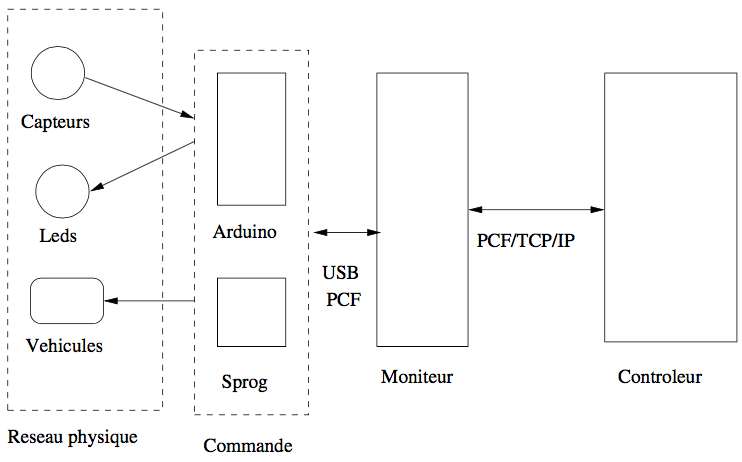
\includegraphics[scale=0.45]{include/communication.png}
\end{frame}

%----------------------------------------------------

\begin{frame}
  \frametitle{Objectifs}
  Placé dans le cadre de la spécification fournie par nos encadrants, ce projet STL
  a pour objectifs :
  \vspace{1em}
  \begin{enumerate}
  \item Conception d'un système de communication contrôleur/moniteur
    \vspace{1em}
  \item Conception d'un système de gestion des règles de circulation
    \vspace{1em}
  \item Implémentation d'une interface graphique
    \vspace{1em}
  \item Tester le contrôleur sur un circuit réel
  \end{enumerate}
\end{frame}

\begin{frame}
  \frametitle{Organisation}
  Nous pouvons présenter l'organisation de ce projet, en développant les trois points suivant :
  \vspace{1em}
  \begin{itemize}
  \item Travail collaboratif
    \vspace{1em}
  \item Planning
    \vspace{1em}
  \item Réunions
  \end{itemize}
\end{frame}



\begin{frame}
  \frametitle{Système de communication contrôleur/moniteur}
  \framesubtitle{PCF et objet PCF}
  \begin{itemize}
  \item Protocole de contrôle ferroviaire
    \vspace{1em}
    \begin{itemize}
      \item Format XML
        \vspace{1em}
      \item Balises à identifiant unique
        \vspace{1em}
    \end{itemize}
  \item Objet PCF
    \vspace{1em}
    \begin{itemize}
      \item Éléments décrivants un équipement
        \vspace{1em}
      \item Éléments pour la topographie d'un réseau
        \vspace{1em}
      \item Élément pour l'initialisation
        \vspace{1em}
    \end{itemize}
  \end{itemize}
\end{frame}

%----------------------------------------------------

\begin{frame}
  \frametitle{Architecture de la solution}
  \framesubtitle{Diagramme de composant 1}
  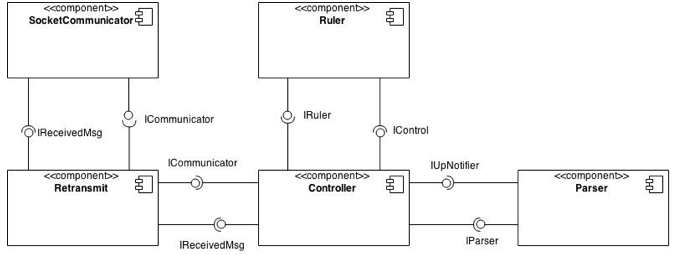
\includegraphics[scale=0.45]{include/diagrammeComposant1.png}
\end{frame}

\begin{frame}
  \frametitle{Architecture de la solution}
  \framesubtitle{Diagramme de composant 2 (final)}
  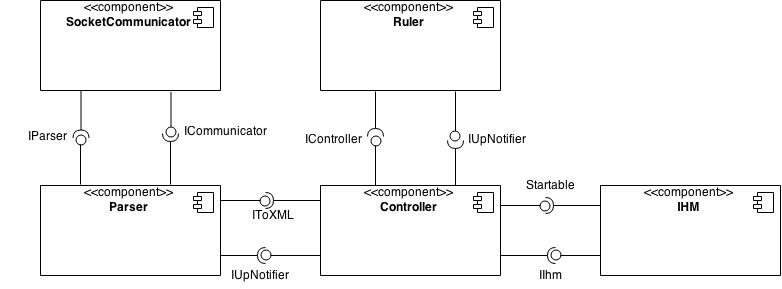
\includegraphics[scale=0.44]{include/diagrammeComposant2.jpg}
\end{frame}

%----------------------------------------------------

\begin{frame}
  \frametitle{Système de communication contrôleur/moniteur}
  \framesubtitle{Les phases des échanges contrôleur/moniteur}
  \begin{columns}[t]
    \begin{column}{0.5\textwidth}
      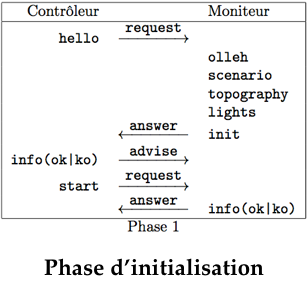
\includegraphics[scale=0.40]{include/phaseInit.png}
    \end{column}
    \begin{column}{0.5\textwidth}
      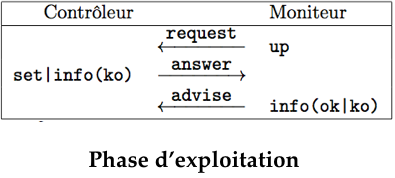
\includegraphics[scale=0.40]{include/phaseExpl.png}
    \end{column}
  \end{columns}
\end{frame}

%----------------------------------------------------

\begin{frame}
  \frametitle{Système de gestion des règles de circulation}
  \framesubtitle{1er Scénario}
  Circuit minimal
  \vspace{1em}
  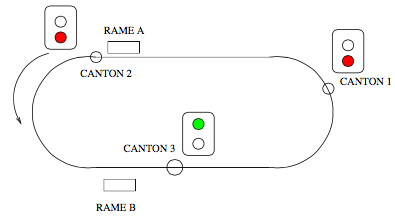
\includegraphics[scale=0.70]{include/scenario1.png}
\end{frame}

\begin{frame}
  \frametitle{Système de gestion des règles de circulation}
  \framesubtitle{2ème Scénario}
  Ajout des aiguillages 2-1
  \vspace{1em}
  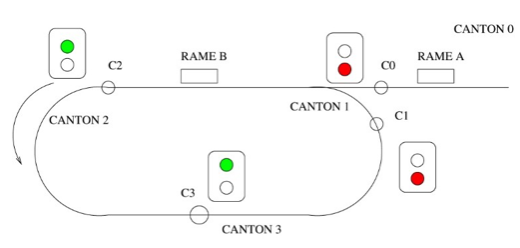
\includegraphics[scale=0.65]{include/scenario2.png}
\end{frame}

\begin{frame}
  \frametitle{Système de gestion des règles de circulation}
  \framesubtitle{3ème Scénario}
  Ajout des aiguillages 1-2 et des stations
  \vspace{1em}
  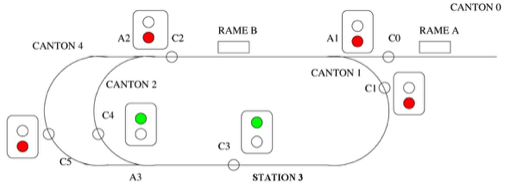
\includegraphics[scale=0.60]{include/scenario3.png}
\end{frame}

%----------------------------------------------------

\begin{frame}
  \frametitle{Interface graphique}
  \framesubtitle{Statique}
  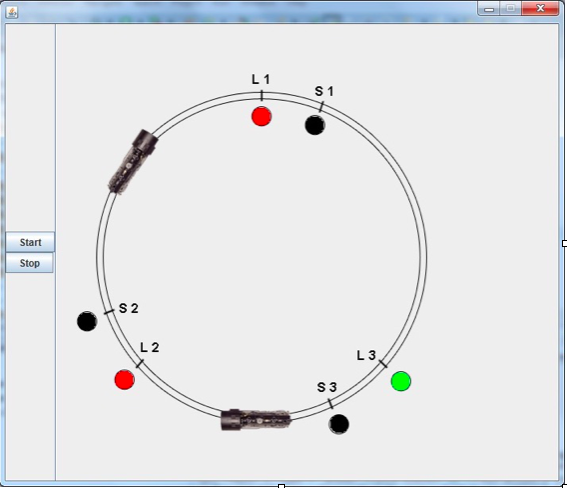
\includegraphics[scale=0.45]{include/ihmStat.png}
\end{frame}

%----------------------------------------------------

\begin{frame}
  \frametitle{Interface graphique}
  \framesubtitle{Dynamique}
  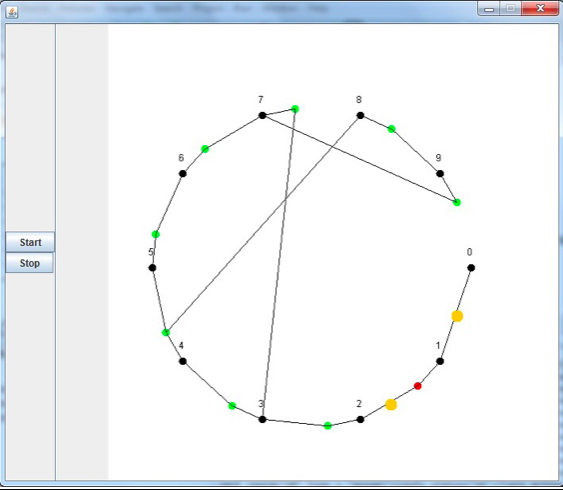
\includegraphics[scale=0.45]{include/ihmDyn.png}
\end{frame}


%---------------------------------------------------------

\begin{frame}
\frametitle{Conclusion}
\begin{enumerate}
  \visible<1->{
  \item Réalisations
    \begin{itemize}
    \item Réalisation du contrôleur
    \item Réalisation de l'interface graphique de l'application
    \item Test de l'application sur un circuit réel
    \end{itemize}
  }
  \visible<2->{
  \item Travail à long terme
    \begin{itemize}
      \item Faire une interface de commande complete
      \item Prendre en compte plus de contraintes
    \end{itemize}
  }
  \visible<3->{
  \item Des questions ?
  }
\end{enumerate}
\end{frame}

\end{document}
